\documentclass{article}
\usepackage[utf8]{inputenc}
\usepackage{geometry, mathtools, dsfont, listings, color, float}

\definecolor{mygreen}{RGB}{28,172,0} % color values Red, Green, Blue
\definecolor{mylilas}{RGB}{170,55,241}

\title{Rendezvous Documentation}
\author{Paul Glotfelter}
\date{March 26, 2016}

\geometry{margin = 0.75in}

\begin{document}

\maketitle

\section{Introduction}

This document is a mathematical companion to the rendezvous sample code for the Robotarium.  It summarizes the mathematics behind the consensus algorithm and highlights the transfer of the formal specification to the Robotarium's MATLAB API.  Additionally, this document contains experimental data from the Robotarium's robots. 

\section{Problem Statement} 

Consider a group of $N$ agents, where we define the state of each agent as $x_{i} \in \mathds{R}^{2},~ i = 1,\hdots,N$.  This particular algorithm models each agent with the single-integrator dynamics
\[
\dot{x}_{i} = u_{i}
\]
where $u_{i} \in \mathds{R}^{2}$ is the control input to agent $i$.  The rendezvous problem requires the design of a control input $u_{i}$ such that 
\begin{equation}
    \lim_{t \to \infty} (x_{i} - x_{j}) = 0, ~ \forall ~ i,j = 1,\hdots,N
    \label{eq:solution}
\end{equation}

\section{Solution}
A common solution to the rendezvous problem is to let $u_{i}$ be defined using the local interaction rule (e.g., as in \cite{jadbabaie}).
\[
u_{i} = \sum_{j \in N_{i}} (x_{j} - x_{i})
\]
yielding the node-level dynamics
\begin{equation}
    \dot{x}_{i} = \sum_{j \in N_{i}} (x_{j} - x_{i})
    \label{eq:node-level-dynamics}
\end{equation}
where $N_{i}$ represents the neighbors of agent $i$ induced by a particular communication topology.  For this algorithm, consider the communication topology of the agents to be static and represented by an undirected graph $G = (V, E)$ where the following condition holds 
\[
j \in N_{i} \iff (i, j), (j, i) \in E
\]
Then, the node-level dynamics may be re-written as ensemble-level dynamics by combining the agents' states together into the vector
\[
x = \left[ x_{1,1} ~ x_{2,1} \hdots ~ x_{N,1} ~ x_{1, 2} ~ x_{2, 2} ~ \hdots ~ x_{N, 2} \right]^{T}
\]
yielding the ensemble-level dynamics 
\[
\dot{x} = -(I \otimes L)x
\]
where $L$ is the graph Laplacian to the graph $G$, and $I$ is an identity matrix of the appropriate dimension.  Note that $x_{i, j}$ refers to the $j$th state variable of agent $x_{i} \in \mathds{R}^{2}$.  This algorithm is known as the consensus algorithm.  Using the properties of $L$, we can also show each agent's final position is given by
\[
\lim_{t \to \infty} x_{i}(t) = \dfrac{1}{N} \sum_{j=1}^{N} x_{j}(0), ~ \forall ~ i = 1,\hdots,N
\]
where $x_{j}(0)$ is the initial condition of agent $j$.  This result solves the problem stated in equation~(\ref{eq:solution}).  Interestingly, the agents always meet at the average of the initial conditions.  For relevant properties of the graph Laplacian, refer to sources such as \cite{godsil}.  

% \section{Analysis}

% There exist many well-known properties of the graph Laplacian, as can be found in \cite{godsil}.  In particular, the graph Laplacian has the property
% \[
% \text{null}(G) = \text{span}(\mathds{1})
% \]
% where $\mathds{1}$ is a vector containing only values of 1, if $G$ is connected.  Thus, we know that the state of the agents is driven to $\text{span}(\mathds{1})$, if the graph $G$ is connected for all time.  We can also show that the final positions of the agents are given by
% \[
% \lim_{t \to \infty} x(t) = \dfrac{1}{N} \mathds{1}\mathds{1}^{T} x_{0}
% \]
% where $x_{0}$ is the initial conditions of the agents.  This result solves the problem stated in Equation~\ref{eq:solution}.  Interestingly, the agents meet at the average of the initial conditions.

\section{Implementation} 

Using the previously defined algorithm and the Robotarium's provided MATLAB interface, we implemented the consensus algorithm in equation~(\ref{eq:node-level-dynamics}).  The code snippet below demonstrates the transfer of the consensus algorithm into the Robotarium's MATLAB API.
\lstset{language=Matlab,%
    %basicstyle=\color{red},
    breaklines=true,%
    morekeywords={matlab2tikz},
    keywordstyle=\color{blue},%
    morekeywords=[2]{1}, keywordstyle=[2]{\color{black}},
    identifierstyle=\color{black},%
    stringstyle=\color{mylilas},
    commentstyle=\color{mygreen},%
    showstringspaces=false,%without this there will be a symbol in the places where there is a space
    numbers=left,%
    numberstyle={\tiny \color{black}},% size of the numbers
    numbersep=9pt, % this defines how far the numbers are from the text
    emph=[1]{for,end,break},emphstyle=[1]\color{red}, %some words to emphasise
    %emph=[2]{word1,word2}, emphstyle=[2]{style},    
}
\lstinputlisting[language=Matlab]{code/consensus.m}
For the complete implementation, refer to the Robotarium website.  

\section{Deployment}
For the experiment, we selected $N = 6$ and $G = C_{6}$ (i.e., an undirected cycle graph containing 6 agents).  This choice for $G$ ensured that the agents remained connected during the experiment.  Deploying the consensus algorithm onto the Robotarium yielded the results shown in Figure~\ref{fig:consensus-data}.  Note that, due to the physical size of the robots, the agents did not reach the same point.
\begin{figure}[!ht]
    \centering
    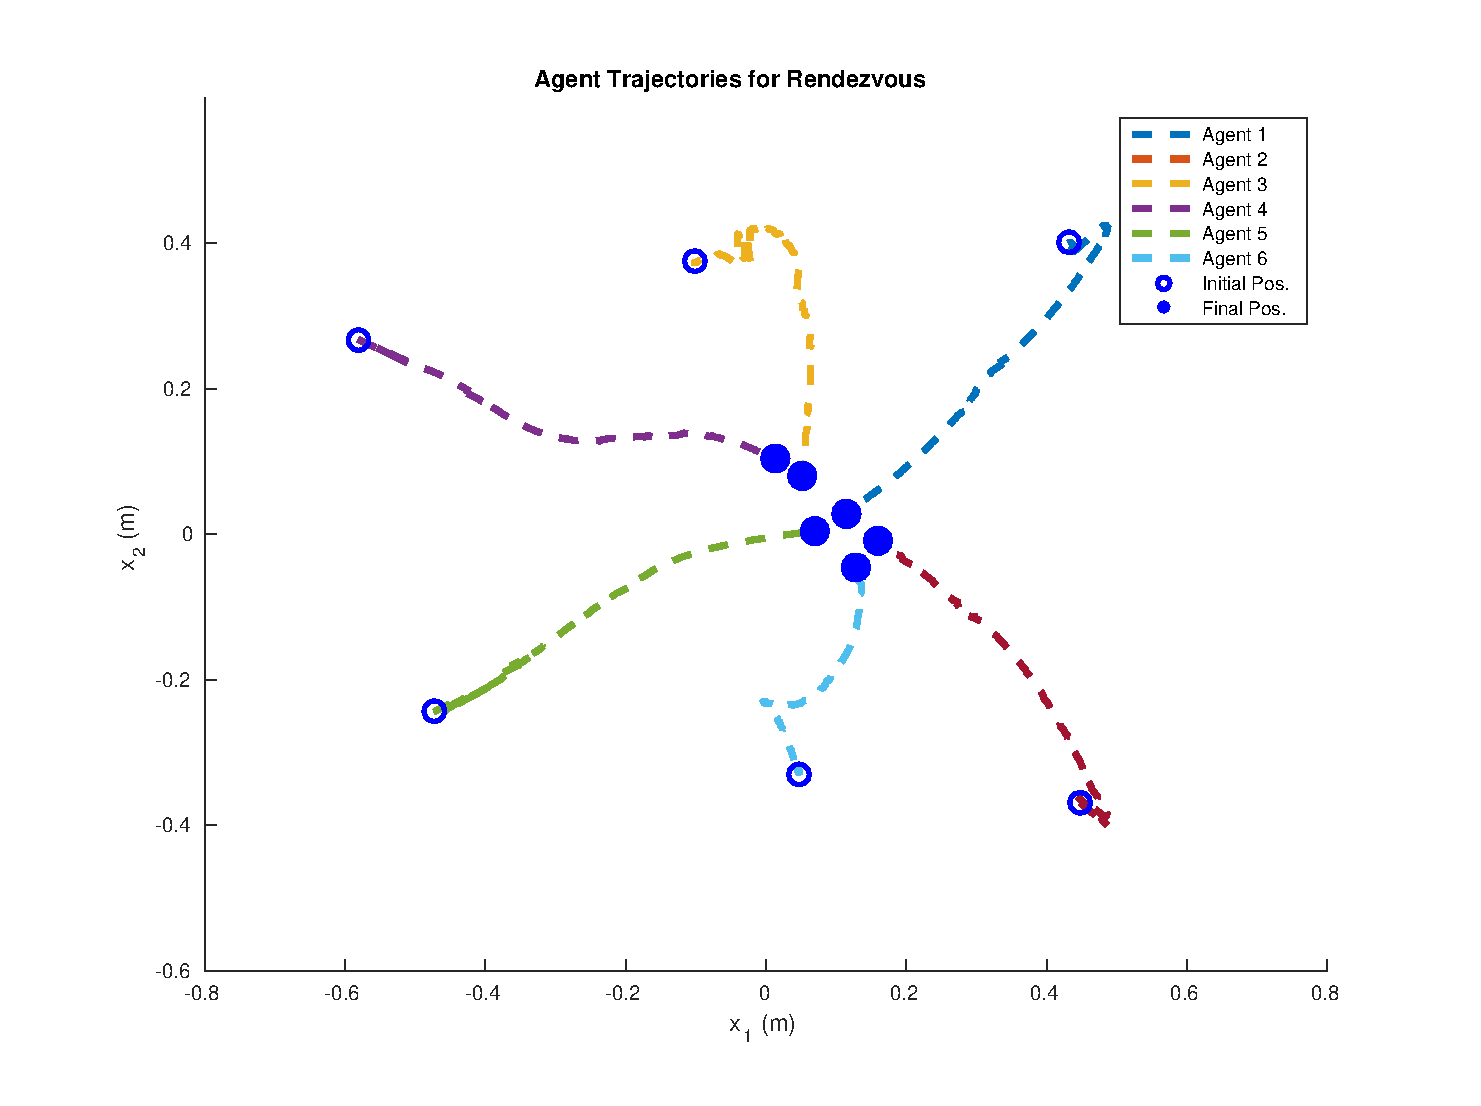
\includegraphics[width=0.7\textwidth]{figures/rendezvous.eps}
    \caption{Physical robots' trajectories during the deployment of the consensus algorithm onto the Robotarium}
    \label{fig:consensus-data}
\end{figure}

\newpage 

\begin{thebibliography}{9}

\bibitem{jadbabaie}
A. Jadbabaie, J. Lin, and A. S. Morse, “Coordination of groups of mobile
autonomous agents using nearest neighbor rules,” \textit{IEEE Trans. Autom. Control}, vol. 48, no. 6, pp. 988–1001, Jun. 2003

\bibitem{godsil}
C. Godsil and G. Royle, \textit{Algebraic Graph Theory}. Berlin, Germany:
Springer, 2001

\end{thebibliography}


\end{document}
